L'evoluzione delle tecnologie legate al Big Data e all'apprendimento automatico ha innescato una vera e propria rivoluzione nei modi in cui i dati vengono gestiti, analizzati e sfruttati. 
La crescente complessità di queste metodologie è emersa come un elemento cruciale, consentendo non solo alle grandi imprese, ma anche a quelle di dimensioni più contenute, di personalizzare in modo avanzato le proprie strategie di marketing proattivo. \\
L'analisi del comportamento del cliente, basata su algoritmi predittivi sofisticati, ha raggiunto un livello di precisione tale da anticipare non solo le esigenze, ma anche i desideri del cliente.
Ciò ha aperto la strada a un'offerta di prodotti e servizi altamente personalizzati. 
Settori come quello bancario e finanziario hanno subito profonde trasformazioni, abbandonando l'approccio tradizionale delle filiali fisiche in favore di servizi di home banking e digitalizzazione completa.
Questa transizione ha migliorato non solo l'accessibilità e l'efficienza dei servizi, ma ha anche generato un ricco patrimonio informativo. \\
L'utilizzo di algoritmi di intelligenza artificiale assiste ora i clienti non solo nella scelta degli investimenti, ma anche nell'implementazione di soluzioni immediate attraverso l'impiego di chatbot avanzati.

Nel campo della ricerca, la bioinformatica ha vissuto una rivoluzione grazie alle nuove tecniche di sequenziamento del DNA. 
Questo progresso ha portato a un'abbondanza di dati genomici, riducendo drasticamente i costi e i tempi necessari per acquisirli. 
L'analisi di questo vasto patrimonio genetico attraverso algoritmi avanzati ha aperto nuove prospettive nella classificazione automatica e nella previsione di indicatori medici, consentendo una comprensione più approfondita della complessità biologica. \\
L'enorme quantità di dati disponibili ha spinto l'analisi avanzata verso l'adozione di tecniche di data mining sempre più sofisticate.
Tuttavia, questa crescita esponenziale ha portato con sé sfide significative, come la diversità dei dati, il loro volume considerevole e l'esigenza di scalabilità per fronteggiare richieste dinamiche. 
Ciò ha stimolato l'innovazione in architetture e modelli di analisi dati, con una transizione da soluzioni tradizionali enterprise a approcci più agili e adattabili. \\
Il punto di partenza per ciò che oggi consideriamo come Big Data può essere fatto risalire al 2004 con l'introduzione del paradigma di programmazione MapReduce da parte dei ricercatori di Google, Jeffrey Dean e Sanjay Ghemawat. 
Questa innovazione, basata sul principio del Divide et Impera, ha rivoluzionato la capacità di elaborazione distribuita, aprendo la strada all'analisi su vasta scala e all'utilizzo efficiente delle risorse in ambienti cloud.

La necessità di elaborare grandi volumi di dati in tempo reale ha dato origine a un'architettura a pipeline. 
Questo modello, in cui ogni componente processa l'output del precedente, è stato plasmato per rispondere alle esigenze di contesti dinamici e mutevoli. 
Le fasi di ingestione, pre-processing, analisi, persistenza e visualizzazione definiscono un approccio strutturato che consente l'analisi continua e dinamica dei dati in tempo reale. \\
Nonostante il consolidato paradigma MapReduce, si è dimostrato insufficiente per affrontare l'elaborazione in tempo reale. 
L'introduzione di nuovi modelli di processamento streaming parallelo, come quelli proposti dalle architetture Lambda e lo stack SMACK, ha rappresentato una tappa fondamentale nell'ottimizzazione delle operazioni di analisi dei Big Data. 
Queste soluzioni offrono efficienza e tempi di risposta più rapidi, garantendo una gestione ottimale dei dati in tempo reale.

\section[Architettura LAMBDA]{Architettura LAMBDA}
L'architettura LAMBDA è frutto dell'ingegno di Nathan Marz, programmatore statunitense noto per aver ideato nel 2011 il framework \textit{Apache Storm} per l'elaborazione in streaming, successivamente acquisito da Twitter.
La concezione di questa architettura è stata presentata nel libro "\textit{Big Data - Principles and best practices of scalable real-time data systems}" \cite{bigDataBook}, in cui l'autore ha proposto un approccio architetturale innovativo, unendo al tradizionale metodo offline (\textit{batch}) delle tecniche di elaborazione online (\textit{streaming}) per il trattamento dei dati in tempo reale.
La tipica architettura Lambda può essere suddivisa in tre strati distinti:
\begin{itemize}
    \item \textbf{Batch Layer}: deputato all'elaborazione batch, tipicamente con paradigma MapReduce, svolgendo anche il compito di persistere il master dataset e garantirne l'allineamento e la consistenza.
    \item \textbf{Speed Layer}: l'elemento di innovazione, deputato al processamento dei dati in tempo reale attingendo dal flusso di input.
    \item \textbf{Serving Layer}: interfaccia verso l'esterno, offre servizi di interrogazione e fornisce in maniera trasparente all'utente un unico virtuale dataset costituito aggregando opportunamente i dati prodotti dalle componenti batch e real time.
\end{itemize}

\begin{figure}[h]
    \centering
    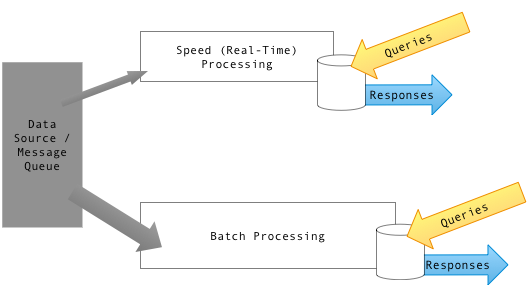
\includegraphics[width = 0.6\textwidth]{diagram_of_lambda_architecture.png}
    \caption[Architettura LAMBDA]{Diagramma di un'architettura LAMBDA \cite{lambdaArchitecture}}
\end{figure}

Il flusso elaborativo è esemplificato dai seguenti passi:
\begin{itemize}
    \item nella fase di \textit{ingestion}, i dati raw vengono catturati in modo simultaneo dalla sorgente. Questi dati alimentano un master dataset che funge da deposito immutabile e aggiornabile solo in modo incrementale, contenendo una copia inalterabile dei dati nel formato originale. Contestualmente, le componenti di processamento in \textit{streaming} vengono attivate per elaborare continuamente i dati in arrivo
    \item durante la fase di processamento, le componenti \textit{batch} intraprendono un approccio di ricalcolo totale o incrementale sul master dataset. Queste operazioni coinvolgono un alto volume di dati, presentano una latenza significativa e hanno un \textit{throughput} relativamente basso. Parallelamente, le componenti \textit{speed} processano lo stesso set di dati acquisito dalle operazioni \textit{batch}, fornendo risultati parziali attraverso tecniche di processamento real-time o pseudo real-time. Questo processo, eseguito a frequenze estremamente elevate e con bassa latenza, offre una visione istantanea e continua del blocco di dati trattato. I risultati ottenuti in questa fase vengono resi disponibili al \textit{Serving Layer}
    \item il \textit{Serving Layer}, infine, agisce come punto di convergenza, aggregando i risultati provenienti sia dalle operazioni \textit{batch} che da quelle in \textit{streaming}. Il suo ruolo principale è quello di fornire un'interfaccia unificata e coerente all'utente finale. Questo strato si occupa inoltre di sovrascrivere eventuali risultati parziali derivanti dall'elaborazione in \textit{streaming} con quelli ottenuti dalle operazioni \textit{batch}, garantendo così una visione complessiva e accurata dei dati trattati. Ad esempio, se nel processing in streaming vengono prodotti risultati parziali per un determinato set di dati, il \textit{Serving Layer} li integra con i risultati ottenuti dalle operazioni \textit{batch} per presentare all'utente una visione completa e aggiornata
\end{itemize}

Questo innovativo modello architetturale introduce notevoli elementi di cambiamento.
Innanzitutto, la mutabilità gestita tradizionalmente all'interno dei database enterprise viene sostituita dall'immutabilità del master dataset, il quale preserva la storia inalterata nel tempo nella sua forma originale.
Aggiunge continuamente nuovi flussi di dati senza mai rimuovere quelli precedenti.
I due strati si compensano reciprocamente in modo trasparente per gli utenti finali, offrendo una visione completa dei dati trattati.
Tale visione deriva da analisi approfondite sui dati storici e fornisce insight e statistiche parziali sui dati attuali.
Il master dataset persiste tipicamente utilizzando file system distribuiti (come \textit{Apache HDFS}) o database distribuiti \textit{NoSQL} (come \textit{MongoDB} orientato ai documenti, \textit{Redis} basato su chiavi, \textit{Neo4J} orientato ai grafi).
La combinazione di calcolo e storage parallelo distribuito consente di massimizzare il principio di località del dato.
Ciò implica il coordinamento e la distribuzione dell'elaborazione e del carico computazionale verso i nodi di lavoro che ospitano i blocchi di dati da elaborare.
Nel contesto di questa architettura, i principali framework di riferimento includono \textit{Apache Hadoop} \cite{hadoop} e \textit{Apache Spark} \cite{spark} per le componenti \textit{batch}, mentre per le componenti \textit{streaming} sono menzionati \textit{Apache Storm} e \textit{Spark Streaming}, che fa parte dell'ecosistema di \textit{Spark}.

\section[Stack SMACK]{Lo Stack SMACK}
La stack \textit{SMACK} è un insieme di tecnologie open source progettato per gestire e analizzare grandi volumi di dati in tempo reale.
L'acronimo \textit{SMACK} rappresenta le principali componenti dello stack: \textit{Spark}, \textit{Mesos}, \textit{Akka}, \textit{Cassandra} e \textit{Kafka}.
Ogni componente svolge un ruolo cruciale nel garantire una gestione efficiente, scalabile e resiliente dei dati.

\begin{figure}[!ht]
    \centering
    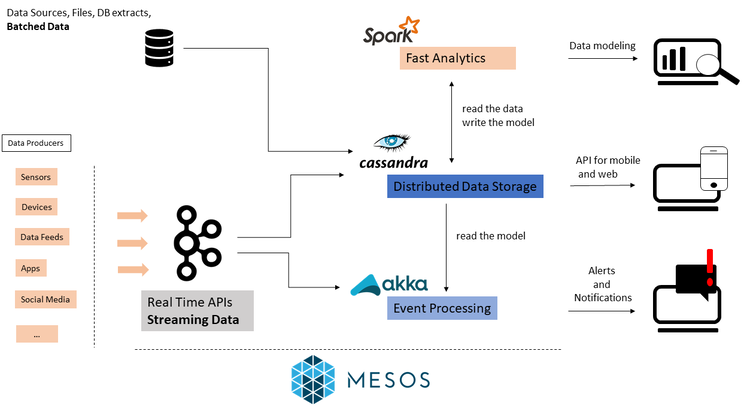
\includegraphics[width=0.6\textwidth]{smack.png}
    \caption[Stack SMACK]{Architettura dello Stack SMACK \cite{smack}}
\end{figure}

Analizziamo ogni componente:
\begin{itemize}
    \item \textbf{Apache Spark}: un framework di elaborazione distribuita che offre un modello di programmazione flessibile e veloce. 
    Spark facilita l'analisi di dati in tempo reale e fornisce un'interfaccia per il processing batch, streaming, SQL e machine learning. 
    La sua architettura a DAG (Directed Acyclic Graph) consente una pipeline di lavoro ottimizzata, promuovendo la velocità e la scalabilità.
    \begin{itemize}
        \item Modello di Programmazione Resiliente a Fallimenti (\textit{RDD}): Spark utilizza un modello di programmazione chiamato Resilient Distributed Dataset (\textit{RDD}). Gli \textit{RDD} sono collezioni distribuite di oggetti immutabili che possono essere elaborati in parallelo. Questo modello fornisce una gestione automatica dei fallimenti, consentendo a Spark di tollerare la perdita di dati durante l'elaborazione.
        \item \textit{Spark Core}: Questo è il nucleo del framework e fornisce le funzionalità di base di Spark, inclusa l'implementazione degli \textit{RDD} e l'engine di esecuzione distribuita. Spark Core è responsabile della gestione delle risorse, della tolleranza ai guasti e dell'interazione con lo storage distribuito.
        \item \textit{Spark SQL}: Questo modulo consente l'elaborazione di dati strutturati utilizzando SQL in Spark. Fornisce un'interfaccia per l'interrogazione dei dati attraverso comandi SQL standard, consentendo agli utenti di eseguire query su dati strutturati insieme alle elaborazioni batch e streaming.
        \item \textit{Spark Streaming}: È un modulo di Spark che consente l'elaborazione di dati in tempo reale. Utilizzando intervalli di microbatching, Spark Streaming elabora i dati in piccoli lotti, offrendo una soluzione per l'analisi dei dati in streaming senza dover ricorrere a un sistema separato.
        \item \textit{MLlib} (Machine Learning Library): Questa libreria integrata in Spark offre un'ampia gamma di algoritmi di machine learning scalabili. È progettata per semplificare lo sviluppo e l'implementazione di modelli di machine learning su grandi dataset distribuiti.
        \item \textit{GraphX}: È una libreria per l'elaborazione di grafi e l'analisi di dati basati su grafi. Grazie a GraphX, Spark può gestire in modo efficiente operazioni su grafi su scala distribuita, rendendolo adatto per applicazioni di social network, analisi delle reti, e altro ancora.
    \end{itemize}
    \item \textbf{Mesos} è un sistema di gestione delle risorse distribuite che fornisce un'astrazione delle risorse della macchina, consentendo l'esecuzione di applicazioni su cluster eterogenei. Mesos offre una gestione dinamica delle risorse, consentendo alle applicazioni di condividere efficientemente risorse come CPU e memoria, rendendo più flessibile l'utilizzo delle infrastrutture.
    
    \begin{figure}[h]
        \centering
        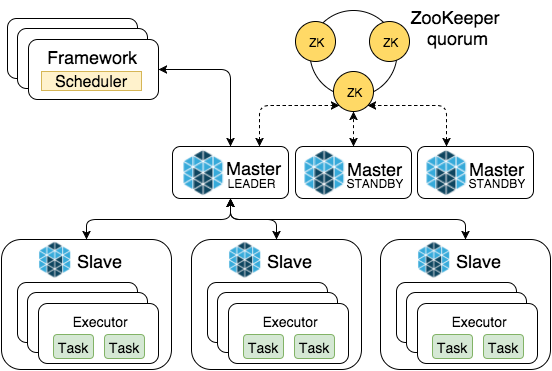
\includegraphics[width = 0.5\textwidth]{mesos.png}
        \caption[Architettura MESOS]{Diagramma dell'architettura di MESOS \cite{mesos}}
    \end{figure}

    \item \textbf{Akka} è un framework per la creazione di sistemi distribuiti e concorrenti basato sul modello di attori. Gli attori sono entità leggere che comunicano tra loro tramite messaggi, consentendo la costruzione di applicazioni altamente scalabili e resilienti. Akka facilita la gestione della concorrenza e fornisce strumenti per affrontare le sfide dei sistemi distribuiti.
    \item \textbf{Apache Cassandra} è un sistema di gestione del database distribuito altamente scalabile e altamente disponibile. Progettato per gestire grandi quantità di dati su cluster di macchine, Cassandra offre una distribuzione automatica dei dati e una replicazione multi-regionale, garantendo l'affidabilità e la resilienza del sistema anche in caso di guasti hardware o nodi inattivi.
    \item \textbf{Apache Kafka} è una piattaforma di streaming distribuito per la gestione di feed di dati in tempo reale. Kafka consente la pubblicazione e il consumo di eventi su larga scala, garantendo la robustezza e l'affidabilità delle pipeline di dati in tempo reale. La sua architettura a \textit{topic} consente una facile scalabilità e gestione dei flussi di dati.
\end{itemize}

Insieme, queste tecnologie formano la stack SMACK, offrendo una soluzione completa per l'elaborazione e l'analisi di dati in tempo reale su scala distribuita.
La combinazione sinergica di Spark, Mesos, Akka, Cassandra e Kafka fornisce un ambiente potente e flessibile per affrontare le sfide dell'analisi dei big data in tempo reale.